\section{Introduction}
\label{sec:intro}

\begin{figure*}[!ht]
    \centering
    \vspace{-3mm}
	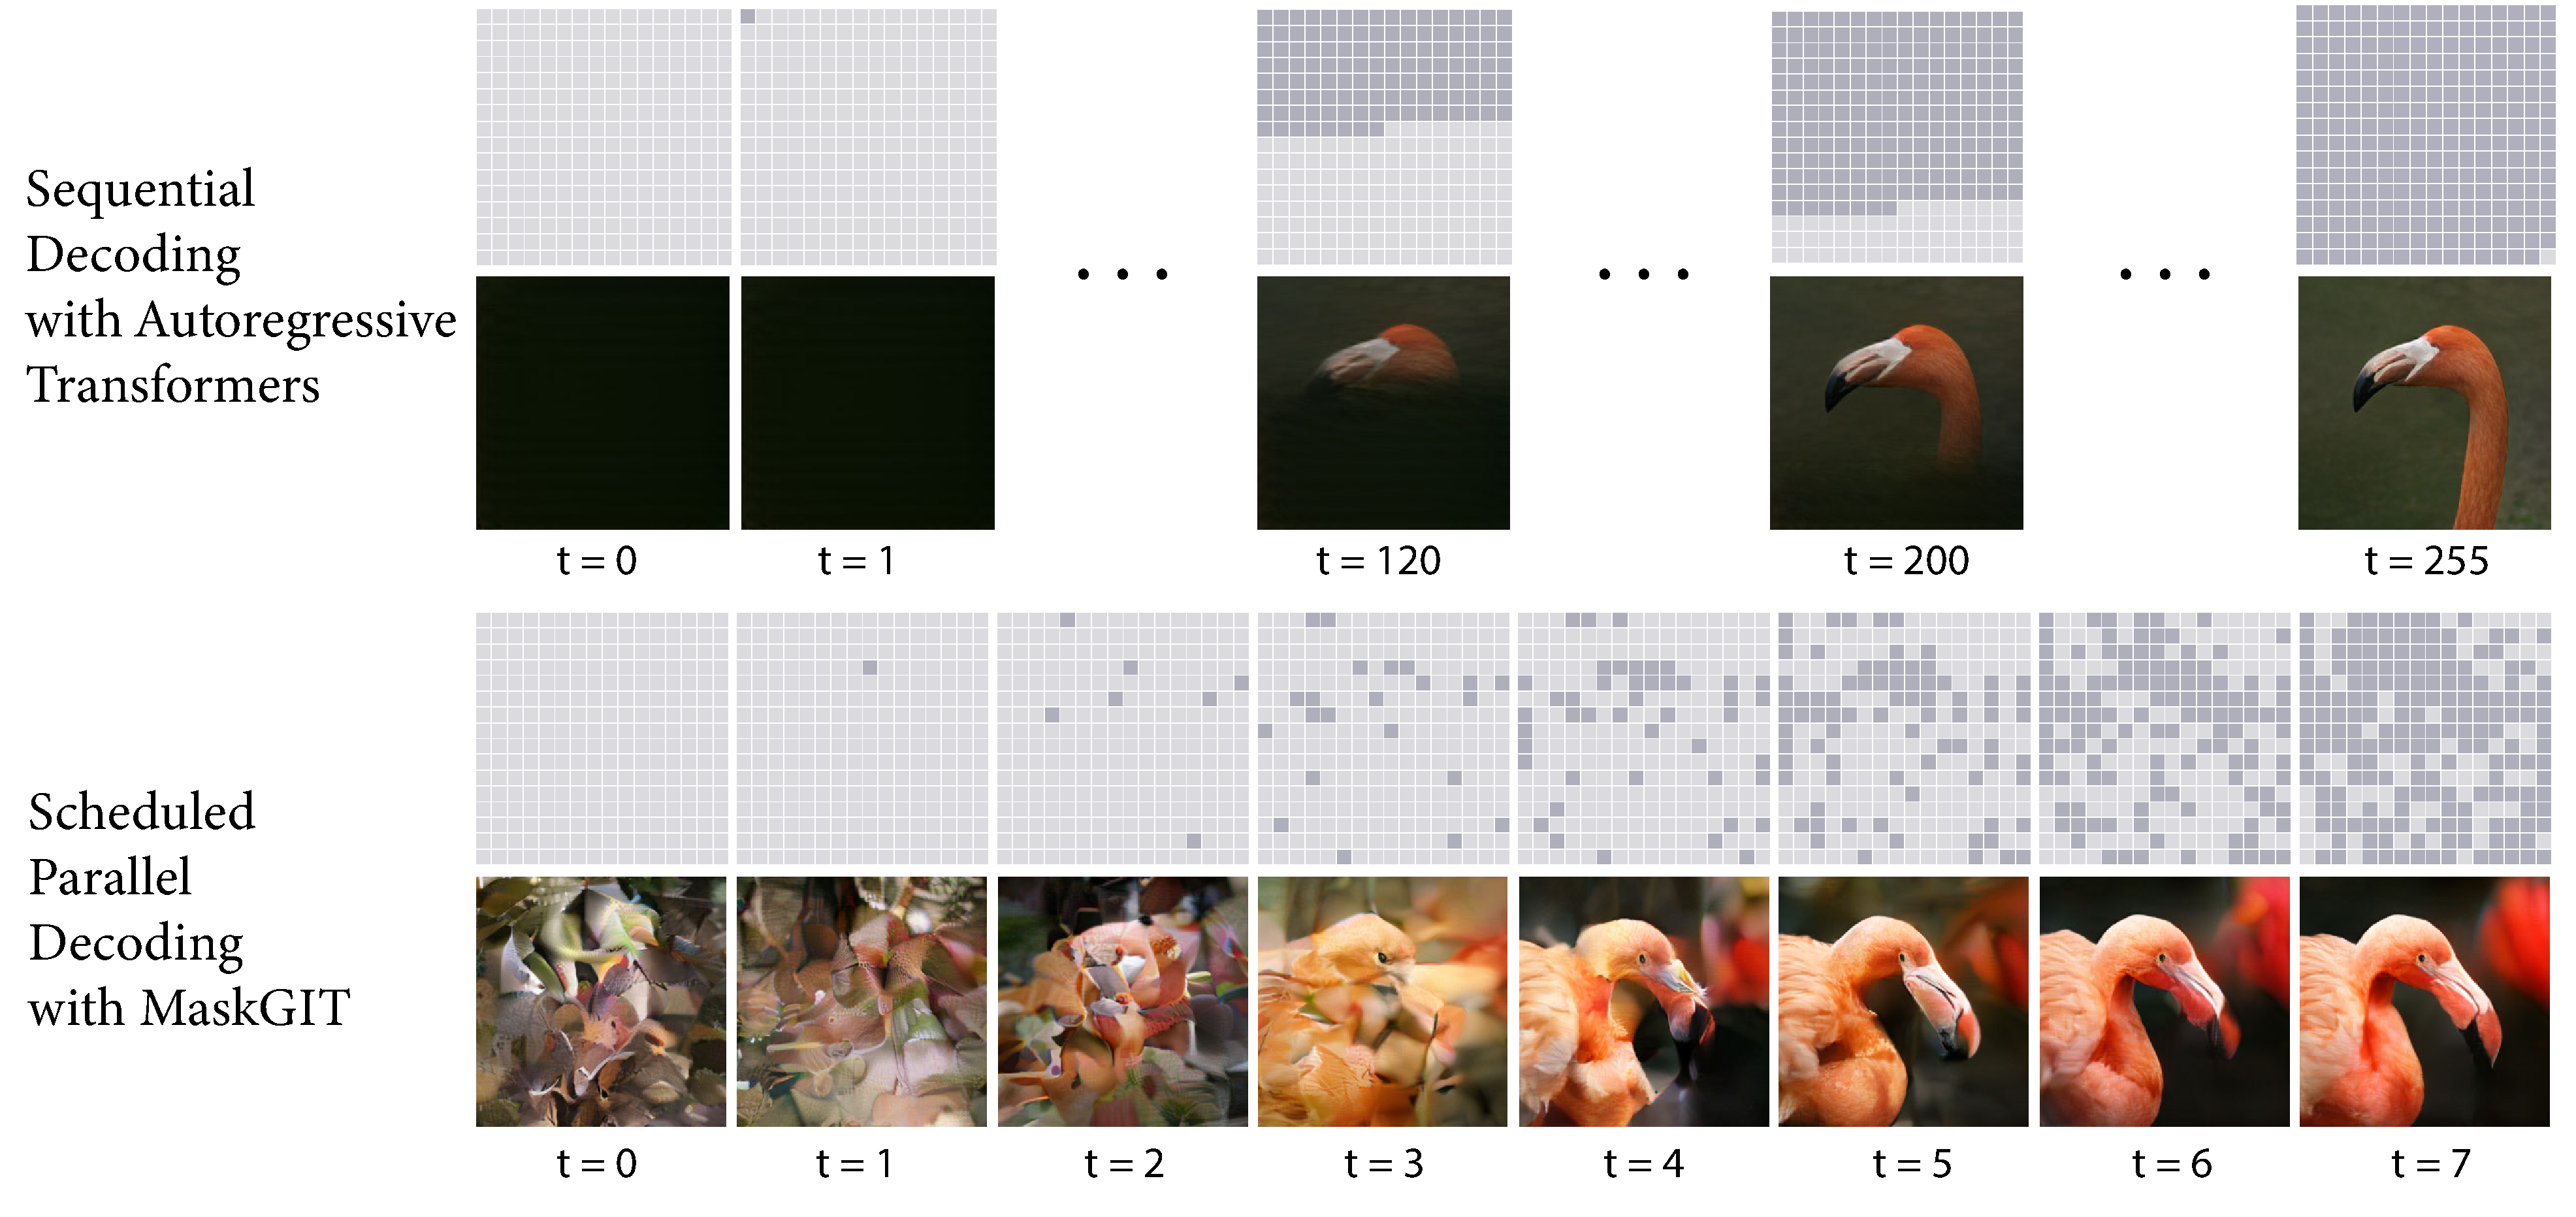
\includegraphics[width=.9\textwidth]{figures/iterative_decoding.pdf}
    \vspace{-3mm}
    \caption{\textbf{Comparison between sequential decoding and \model's scheduled parallel decoding.} Rows 1 and 3 are the input latent masks at each iteration, and rows 2 and 4 are samples generated by each model at that iteration. Our decoding starts with all unknown codes (marked in lighter gray), and gradually fills up the latent representation with more and more scattered predictions in parallel (marked in darker gray), where the number of predicted tokens increases sharply over iterations. \model finishes its decoding in 8 iterations compared to the 256 rounds the sequential method takes.}
    \label{fig:decoding}
\vspace{-3mm}
\end{figure*}


Deep image synthesis as a field has seen a lot of progress in recent years. Currently holding state-of-the-art results are Generative Adversarial Networks (GANs), which are capable of synthesizing high-fidelity images at blazing speeds. They suffer from, however, well known issues include training instability and mode collapse, which lead to a lack of sample diversity. Addressing these issues still remains open research problems.

Inspired by the success of Transformer~\cite{Vaswani17attention} and GPT~\cite{gpt3} in NLP, generative transformer models have received  growing interests in image synthesis~\cite{chen2020imagegpt,Esser21vqgan,Razavi19vqvae2}. Generally, these approaches aim at modeling an image like a sequence and leveraging the existing autoregressive models to generate image. Images are generated in two stages; the first stage is to quantize an image to a sequence of discrete tokens (or visual words). In the second stage, an autoregressive model (e.g., transformer) is learned to generate image tokens sequentially based on the previously generated result (\ie autoregressive decoding). Unlike the subtle min-max optimization used in GANs, these models are learned by maximum likelihood estimation. Because of the design differences, existing works have demonstrated their advantages over GANs in offering stabilized training and improved distribution coverage or diversity.

Existing works on generative transformers mostly focus on the first stage, \ie how to quantize images such that information loss is minimized, and share the same second stage borrowed from NLP. Consequently, even the state-of-the-art generative transformers~\cite{Esser21vqgan,Ramesh21dalle} still treat an image naively as a sequence, where an image is flattened into a 1D sequence of tokens following a raster scan ordering, \ie from left to right line-by-line (\cf Figure~\ref{fig:decoding}). We find this representation neither optimal nor efficient for images. Unlike text, images are not sequential. Imagine how an artwork is created. A painter starts with a sketch and then progressively refines it by filling or tweaking the details, which is in clear contrast to the line-by-line printing used in previous work~\cite{chen2020imagegpt,Esser21vqgan}. Additionally, treating image as a flat sequence means that the autoregressive sequence length grows quadratically, easily forming an extremely long sequence--longer than any natural language sentence. This poses challenges for not only modeling long-term correlation but also renders the decoding intractable.  For example, it takes a considerable 30 seconds to generate a single image on a GPU autoregressively with 32x32 tokens.

This paper introduces a new bidirectional transformer for image synthesis called Masked Generative Image Transformer (\model). During training, \model is trained on a similar proxy task to the mask prediction in BERT~\cite{Devlin19bert}. At inference time, \model adopts a novel non-autoregressive decoding method to synthesize an image in constant number of steps. Specifically, at each iteration, the model predicts all tokens simultaneously in parallel but only keeps the most confident ones. The remaining tokens are masked out and will be re-predicted in the next iteration. The mask ratio is decreased until all tokens are generated with a few iterations of refinement. As illustrated in Figure~\ref{fig:decoding}, \model's decoding is an order-of-magnitude faster than the autoregresive decoding as it only takes 8 steps, instead of 256 steps, to generate an image and the predictions within each step are parallelizable. Moreover, instead of conditioning only on previous tokens in the order of raster scan, bidirectional self-attention allows the model to generate new tokens from generated tokens in all directions. We find that the mask scheduling (\ie fraction of the image masked each iteration) significantly affects generation quality. We propose to use the cosine schedule and substantiate its efficacy in the ablation study.

On the ImageNet benchmark, we empirically demonstrate that \model is both significantly faster (by up to 64x) and capable of generating higher quality samples than the state-of-the-art autoregressive transformer, \ie VQGAN, on class-conditional generation with 256$\times$256 and 512$\times$512 resolution. Even compared with the leading GAN model, \ie BigGAN, and diffusion model, \ie ADM~\cite{dhariwal2021diffusion}, \model offers comparable sample quality while yielding more favourable diversity. Notably, our model establishes new state-of-the-arts on classification accuracy score (CAS)~\cite{Ravuri19CAS} and on FID\cite{FID} for synthesizing 512$\times$512 images. To our knowledge, this paper provides the first evidence demonstrating the efficacy of the masked modeling for image generation on the common ImageNet benchmark.  

Furthermore, MaskGIT's multidirectional nature makes it readily extendable to image manipulation tasks that are otherwise difficult for autoregressive models. Fig.~\ref{fig:teaser} shows a new application of class-conditional image editing in which \model re-generates content inside the bounding box based on the given class while keeping the context (outside of the box) unchanged. This task, which is either infeasible for autoregressive model or difficult for GAN models, is trivial for our model.
Quantitatively, we demonstrate this flexibility by applying \model to image inpainting, and image extrapolation in arbitrary directions.
%shown in Fig.~\ref{fig:teaser}
Even though our model is not designed for such tasks, it obtains comparable performance to the dedicated models on each task.

